
% Default to the notebook output style

    


% Inherit from the specified cell style.




    
\documentclass[11pt]{article}

    
    
    \usepackage[T1]{fontenc}
    % Nicer default font (+ math font) than Computer Modern for most use cases
    \usepackage{mathpazo}

    % Basic figure setup, for now with no caption control since it's done
    % automatically by Pandoc (which extracts ![](path) syntax from Markdown).
    \usepackage{graphicx}
    % We will generate all images so they have a width \maxwidth. This means
    % that they will get their normal width if they fit onto the page, but
    % are scaled down if they would overflow the margins.
    \makeatletter
    \def\maxwidth{\ifdim\Gin@nat@width>\linewidth\linewidth
    \else\Gin@nat@width\fi}
    \makeatother
    \let\Oldincludegraphics\includegraphics
    % Set max figure width to be 80% of text width, for now hardcoded.
    \renewcommand{\includegraphics}[1]{\Oldincludegraphics[width=.8\maxwidth]{#1}}
    % Ensure that by default, figures have no caption (until we provide a
    % proper Figure object with a Caption API and a way to capture that
    % in the conversion process - todo).
    \usepackage{caption}
    \DeclareCaptionLabelFormat{nolabel}{}
    \captionsetup{labelformat=nolabel}

    \usepackage{adjustbox} % Used to constrain images to a maximum size 
    \usepackage{xcolor} % Allow colors to be defined
    \usepackage{enumerate} % Needed for markdown enumerations to work
    \usepackage{geometry} % Used to adjust the document margins
    \usepackage{amsmath} % Equations
    \usepackage{amssymb} % Equations
    \usepackage{textcomp} % defines textquotesingle
    % Hack from http://tex.stackexchange.com/a/47451/13684:
    \AtBeginDocument{%
        \def\PYZsq{\textquotesingle}% Upright quotes in Pygmentized code
    }
    \usepackage{upquote} % Upright quotes for verbatim code
    \usepackage{eurosym} % defines \euro
    \usepackage[mathletters]{ucs} % Extended unicode (utf-8) support
    \usepackage[utf8x]{inputenc} % Allow utf-8 characters in the tex document
    \usepackage{fancyvrb} % verbatim replacement that allows latex
    \usepackage{grffile} % extends the file name processing of package graphics 
                         % to support a larger range 
    % The hyperref package gives us a pdf with properly built
    % internal navigation ('pdf bookmarks' for the table of contents,
    % internal cross-reference links, web links for URLs, etc.)
    \usepackage{hyperref}
    \usepackage{longtable} % longtable support required by pandoc >1.10
    \usepackage{booktabs}  % table support for pandoc > 1.12.2
    \usepackage[inline]{enumitem} % IRkernel/repr support (it uses the enumerate* environment)
    \usepackage[normalem]{ulem} % ulem is needed to support strikethroughs (\sout)
                                % normalem makes italics be italics, not underlines
    

    
    
    % Colors for the hyperref package
    \definecolor{urlcolor}{rgb}{0,.145,.698}
    \definecolor{linkcolor}{rgb}{.71,0.21,0.01}
    \definecolor{citecolor}{rgb}{.12,.54,.11}

    % ANSI colors
    \definecolor{ansi-black}{HTML}{3E424D}
    \definecolor{ansi-black-intense}{HTML}{282C36}
    \definecolor{ansi-red}{HTML}{E75C58}
    \definecolor{ansi-red-intense}{HTML}{B22B31}
    \definecolor{ansi-green}{HTML}{00A250}
    \definecolor{ansi-green-intense}{HTML}{007427}
    \definecolor{ansi-yellow}{HTML}{DDB62B}
    \definecolor{ansi-yellow-intense}{HTML}{B27D12}
    \definecolor{ansi-blue}{HTML}{208FFB}
    \definecolor{ansi-blue-intense}{HTML}{0065CA}
    \definecolor{ansi-magenta}{HTML}{D160C4}
    \definecolor{ansi-magenta-intense}{HTML}{A03196}
    \definecolor{ansi-cyan}{HTML}{60C6C8}
    \definecolor{ansi-cyan-intense}{HTML}{258F8F}
    \definecolor{ansi-white}{HTML}{C5C1B4}
    \definecolor{ansi-white-intense}{HTML}{A1A6B2}

    % commands and environments needed by pandoc snippets
    % extracted from the output of `pandoc -s`
    \providecommand{\tightlist}{%
      \setlength{\itemsep}{0pt}\setlength{\parskip}{0pt}}
    \DefineVerbatimEnvironment{Highlighting}{Verbatim}{commandchars=\\\{\}}
    % Add ',fontsize=\small' for more characters per line
    \newenvironment{Shaded}{}{}
    \newcommand{\KeywordTok}[1]{\textcolor[rgb]{0.00,0.44,0.13}{\textbf{{#1}}}}
    \newcommand{\DataTypeTok}[1]{\textcolor[rgb]{0.56,0.13,0.00}{{#1}}}
    \newcommand{\DecValTok}[1]{\textcolor[rgb]{0.25,0.63,0.44}{{#1}}}
    \newcommand{\BaseNTok}[1]{\textcolor[rgb]{0.25,0.63,0.44}{{#1}}}
    \newcommand{\FloatTok}[1]{\textcolor[rgb]{0.25,0.63,0.44}{{#1}}}
    \newcommand{\CharTok}[1]{\textcolor[rgb]{0.25,0.44,0.63}{{#1}}}
    \newcommand{\StringTok}[1]{\textcolor[rgb]{0.25,0.44,0.63}{{#1}}}
    \newcommand{\CommentTok}[1]{\textcolor[rgb]{0.38,0.63,0.69}{\textit{{#1}}}}
    \newcommand{\OtherTok}[1]{\textcolor[rgb]{0.00,0.44,0.13}{{#1}}}
    \newcommand{\AlertTok}[1]{\textcolor[rgb]{1.00,0.00,0.00}{\textbf{{#1}}}}
    \newcommand{\FunctionTok}[1]{\textcolor[rgb]{0.02,0.16,0.49}{{#1}}}
    \newcommand{\RegionMarkerTok}[1]{{#1}}
    \newcommand{\ErrorTok}[1]{\textcolor[rgb]{1.00,0.00,0.00}{\textbf{{#1}}}}
    \newcommand{\NormalTok}[1]{{#1}}
    
    % Additional commands for more recent versions of Pandoc
    \newcommand{\ConstantTok}[1]{\textcolor[rgb]{0.53,0.00,0.00}{{#1}}}
    \newcommand{\SpecialCharTok}[1]{\textcolor[rgb]{0.25,0.44,0.63}{{#1}}}
    \newcommand{\VerbatimStringTok}[1]{\textcolor[rgb]{0.25,0.44,0.63}{{#1}}}
    \newcommand{\SpecialStringTok}[1]{\textcolor[rgb]{0.73,0.40,0.53}{{#1}}}
    \newcommand{\ImportTok}[1]{{#1}}
    \newcommand{\DocumentationTok}[1]{\textcolor[rgb]{0.73,0.13,0.13}{\textit{{#1}}}}
    \newcommand{\AnnotationTok}[1]{\textcolor[rgb]{0.38,0.63,0.69}{\textbf{\textit{{#1}}}}}
    \newcommand{\CommentVarTok}[1]{\textcolor[rgb]{0.38,0.63,0.69}{\textbf{\textit{{#1}}}}}
    \newcommand{\VariableTok}[1]{\textcolor[rgb]{0.10,0.09,0.49}{{#1}}}
    \newcommand{\ControlFlowTok}[1]{\textcolor[rgb]{0.00,0.44,0.13}{\textbf{{#1}}}}
    \newcommand{\OperatorTok}[1]{\textcolor[rgb]{0.40,0.40,0.40}{{#1}}}
    \newcommand{\BuiltInTok}[1]{{#1}}
    \newcommand{\ExtensionTok}[1]{{#1}}
    \newcommand{\PreprocessorTok}[1]{\textcolor[rgb]{0.74,0.48,0.00}{{#1}}}
    \newcommand{\AttributeTok}[1]{\textcolor[rgb]{0.49,0.56,0.16}{{#1}}}
    \newcommand{\InformationTok}[1]{\textcolor[rgb]{0.38,0.63,0.69}{\textbf{\textit{{#1}}}}}
    \newcommand{\WarningTok}[1]{\textcolor[rgb]{0.38,0.63,0.69}{\textbf{\textit{{#1}}}}}
    
    
    % Define a nice break command that doesn't care if a line doesn't already
    % exist.
    \def\br{\hspace*{\fill} \\* }
    % Math Jax compatability definitions
    \def\gt{>}
    \def\lt{<}
    % Document parameters
    \title{batteries\_AL}
    
    
    

    % Pygments definitions
    
\makeatletter
\def\PY@reset{\let\PY@it=\relax \let\PY@bf=\relax%
    \let\PY@ul=\relax \let\PY@tc=\relax%
    \let\PY@bc=\relax \let\PY@ff=\relax}
\def\PY@tok#1{\csname PY@tok@#1\endcsname}
\def\PY@toks#1+{\ifx\relax#1\empty\else%
    \PY@tok{#1}\expandafter\PY@toks\fi}
\def\PY@do#1{\PY@bc{\PY@tc{\PY@ul{%
    \PY@it{\PY@bf{\PY@ff{#1}}}}}}}
\def\PY#1#2{\PY@reset\PY@toks#1+\relax+\PY@do{#2}}

\expandafter\def\csname PY@tok@w\endcsname{\def\PY@tc##1{\textcolor[rgb]{0.73,0.73,0.73}{##1}}}
\expandafter\def\csname PY@tok@c\endcsname{\let\PY@it=\textit\def\PY@tc##1{\textcolor[rgb]{0.25,0.50,0.50}{##1}}}
\expandafter\def\csname PY@tok@cp\endcsname{\def\PY@tc##1{\textcolor[rgb]{0.74,0.48,0.00}{##1}}}
\expandafter\def\csname PY@tok@k\endcsname{\let\PY@bf=\textbf\def\PY@tc##1{\textcolor[rgb]{0.00,0.50,0.00}{##1}}}
\expandafter\def\csname PY@tok@kp\endcsname{\def\PY@tc##1{\textcolor[rgb]{0.00,0.50,0.00}{##1}}}
\expandafter\def\csname PY@tok@kt\endcsname{\def\PY@tc##1{\textcolor[rgb]{0.69,0.00,0.25}{##1}}}
\expandafter\def\csname PY@tok@o\endcsname{\def\PY@tc##1{\textcolor[rgb]{0.40,0.40,0.40}{##1}}}
\expandafter\def\csname PY@tok@ow\endcsname{\let\PY@bf=\textbf\def\PY@tc##1{\textcolor[rgb]{0.67,0.13,1.00}{##1}}}
\expandafter\def\csname PY@tok@nb\endcsname{\def\PY@tc##1{\textcolor[rgb]{0.00,0.50,0.00}{##1}}}
\expandafter\def\csname PY@tok@nf\endcsname{\def\PY@tc##1{\textcolor[rgb]{0.00,0.00,1.00}{##1}}}
\expandafter\def\csname PY@tok@nc\endcsname{\let\PY@bf=\textbf\def\PY@tc##1{\textcolor[rgb]{0.00,0.00,1.00}{##1}}}
\expandafter\def\csname PY@tok@nn\endcsname{\let\PY@bf=\textbf\def\PY@tc##1{\textcolor[rgb]{0.00,0.00,1.00}{##1}}}
\expandafter\def\csname PY@tok@ne\endcsname{\let\PY@bf=\textbf\def\PY@tc##1{\textcolor[rgb]{0.82,0.25,0.23}{##1}}}
\expandafter\def\csname PY@tok@nv\endcsname{\def\PY@tc##1{\textcolor[rgb]{0.10,0.09,0.49}{##1}}}
\expandafter\def\csname PY@tok@no\endcsname{\def\PY@tc##1{\textcolor[rgb]{0.53,0.00,0.00}{##1}}}
\expandafter\def\csname PY@tok@nl\endcsname{\def\PY@tc##1{\textcolor[rgb]{0.63,0.63,0.00}{##1}}}
\expandafter\def\csname PY@tok@ni\endcsname{\let\PY@bf=\textbf\def\PY@tc##1{\textcolor[rgb]{0.60,0.60,0.60}{##1}}}
\expandafter\def\csname PY@tok@na\endcsname{\def\PY@tc##1{\textcolor[rgb]{0.49,0.56,0.16}{##1}}}
\expandafter\def\csname PY@tok@nt\endcsname{\let\PY@bf=\textbf\def\PY@tc##1{\textcolor[rgb]{0.00,0.50,0.00}{##1}}}
\expandafter\def\csname PY@tok@nd\endcsname{\def\PY@tc##1{\textcolor[rgb]{0.67,0.13,1.00}{##1}}}
\expandafter\def\csname PY@tok@s\endcsname{\def\PY@tc##1{\textcolor[rgb]{0.73,0.13,0.13}{##1}}}
\expandafter\def\csname PY@tok@sd\endcsname{\let\PY@it=\textit\def\PY@tc##1{\textcolor[rgb]{0.73,0.13,0.13}{##1}}}
\expandafter\def\csname PY@tok@si\endcsname{\let\PY@bf=\textbf\def\PY@tc##1{\textcolor[rgb]{0.73,0.40,0.53}{##1}}}
\expandafter\def\csname PY@tok@se\endcsname{\let\PY@bf=\textbf\def\PY@tc##1{\textcolor[rgb]{0.73,0.40,0.13}{##1}}}
\expandafter\def\csname PY@tok@sr\endcsname{\def\PY@tc##1{\textcolor[rgb]{0.73,0.40,0.53}{##1}}}
\expandafter\def\csname PY@tok@ss\endcsname{\def\PY@tc##1{\textcolor[rgb]{0.10,0.09,0.49}{##1}}}
\expandafter\def\csname PY@tok@sx\endcsname{\def\PY@tc##1{\textcolor[rgb]{0.00,0.50,0.00}{##1}}}
\expandafter\def\csname PY@tok@m\endcsname{\def\PY@tc##1{\textcolor[rgb]{0.40,0.40,0.40}{##1}}}
\expandafter\def\csname PY@tok@gh\endcsname{\let\PY@bf=\textbf\def\PY@tc##1{\textcolor[rgb]{0.00,0.00,0.50}{##1}}}
\expandafter\def\csname PY@tok@gu\endcsname{\let\PY@bf=\textbf\def\PY@tc##1{\textcolor[rgb]{0.50,0.00,0.50}{##1}}}
\expandafter\def\csname PY@tok@gd\endcsname{\def\PY@tc##1{\textcolor[rgb]{0.63,0.00,0.00}{##1}}}
\expandafter\def\csname PY@tok@gi\endcsname{\def\PY@tc##1{\textcolor[rgb]{0.00,0.63,0.00}{##1}}}
\expandafter\def\csname PY@tok@gr\endcsname{\def\PY@tc##1{\textcolor[rgb]{1.00,0.00,0.00}{##1}}}
\expandafter\def\csname PY@tok@ge\endcsname{\let\PY@it=\textit}
\expandafter\def\csname PY@tok@gs\endcsname{\let\PY@bf=\textbf}
\expandafter\def\csname PY@tok@gp\endcsname{\let\PY@bf=\textbf\def\PY@tc##1{\textcolor[rgb]{0.00,0.00,0.50}{##1}}}
\expandafter\def\csname PY@tok@go\endcsname{\def\PY@tc##1{\textcolor[rgb]{0.53,0.53,0.53}{##1}}}
\expandafter\def\csname PY@tok@gt\endcsname{\def\PY@tc##1{\textcolor[rgb]{0.00,0.27,0.87}{##1}}}
\expandafter\def\csname PY@tok@err\endcsname{\def\PY@bc##1{\setlength{\fboxsep}{0pt}\fcolorbox[rgb]{1.00,0.00,0.00}{1,1,1}{\strut ##1}}}
\expandafter\def\csname PY@tok@kc\endcsname{\let\PY@bf=\textbf\def\PY@tc##1{\textcolor[rgb]{0.00,0.50,0.00}{##1}}}
\expandafter\def\csname PY@tok@kd\endcsname{\let\PY@bf=\textbf\def\PY@tc##1{\textcolor[rgb]{0.00,0.50,0.00}{##1}}}
\expandafter\def\csname PY@tok@kn\endcsname{\let\PY@bf=\textbf\def\PY@tc##1{\textcolor[rgb]{0.00,0.50,0.00}{##1}}}
\expandafter\def\csname PY@tok@kr\endcsname{\let\PY@bf=\textbf\def\PY@tc##1{\textcolor[rgb]{0.00,0.50,0.00}{##1}}}
\expandafter\def\csname PY@tok@bp\endcsname{\def\PY@tc##1{\textcolor[rgb]{0.00,0.50,0.00}{##1}}}
\expandafter\def\csname PY@tok@fm\endcsname{\def\PY@tc##1{\textcolor[rgb]{0.00,0.00,1.00}{##1}}}
\expandafter\def\csname PY@tok@vc\endcsname{\def\PY@tc##1{\textcolor[rgb]{0.10,0.09,0.49}{##1}}}
\expandafter\def\csname PY@tok@vg\endcsname{\def\PY@tc##1{\textcolor[rgb]{0.10,0.09,0.49}{##1}}}
\expandafter\def\csname PY@tok@vi\endcsname{\def\PY@tc##1{\textcolor[rgb]{0.10,0.09,0.49}{##1}}}
\expandafter\def\csname PY@tok@vm\endcsname{\def\PY@tc##1{\textcolor[rgb]{0.10,0.09,0.49}{##1}}}
\expandafter\def\csname PY@tok@sa\endcsname{\def\PY@tc##1{\textcolor[rgb]{0.73,0.13,0.13}{##1}}}
\expandafter\def\csname PY@tok@sb\endcsname{\def\PY@tc##1{\textcolor[rgb]{0.73,0.13,0.13}{##1}}}
\expandafter\def\csname PY@tok@sc\endcsname{\def\PY@tc##1{\textcolor[rgb]{0.73,0.13,0.13}{##1}}}
\expandafter\def\csname PY@tok@dl\endcsname{\def\PY@tc##1{\textcolor[rgb]{0.73,0.13,0.13}{##1}}}
\expandafter\def\csname PY@tok@s2\endcsname{\def\PY@tc##1{\textcolor[rgb]{0.73,0.13,0.13}{##1}}}
\expandafter\def\csname PY@tok@sh\endcsname{\def\PY@tc##1{\textcolor[rgb]{0.73,0.13,0.13}{##1}}}
\expandafter\def\csname PY@tok@s1\endcsname{\def\PY@tc##1{\textcolor[rgb]{0.73,0.13,0.13}{##1}}}
\expandafter\def\csname PY@tok@mb\endcsname{\def\PY@tc##1{\textcolor[rgb]{0.40,0.40,0.40}{##1}}}
\expandafter\def\csname PY@tok@mf\endcsname{\def\PY@tc##1{\textcolor[rgb]{0.40,0.40,0.40}{##1}}}
\expandafter\def\csname PY@tok@mh\endcsname{\def\PY@tc##1{\textcolor[rgb]{0.40,0.40,0.40}{##1}}}
\expandafter\def\csname PY@tok@mi\endcsname{\def\PY@tc##1{\textcolor[rgb]{0.40,0.40,0.40}{##1}}}
\expandafter\def\csname PY@tok@il\endcsname{\def\PY@tc##1{\textcolor[rgb]{0.40,0.40,0.40}{##1}}}
\expandafter\def\csname PY@tok@mo\endcsname{\def\PY@tc##1{\textcolor[rgb]{0.40,0.40,0.40}{##1}}}
\expandafter\def\csname PY@tok@ch\endcsname{\let\PY@it=\textit\def\PY@tc##1{\textcolor[rgb]{0.25,0.50,0.50}{##1}}}
\expandafter\def\csname PY@tok@cm\endcsname{\let\PY@it=\textit\def\PY@tc##1{\textcolor[rgb]{0.25,0.50,0.50}{##1}}}
\expandafter\def\csname PY@tok@cpf\endcsname{\let\PY@it=\textit\def\PY@tc##1{\textcolor[rgb]{0.25,0.50,0.50}{##1}}}
\expandafter\def\csname PY@tok@c1\endcsname{\let\PY@it=\textit\def\PY@tc##1{\textcolor[rgb]{0.25,0.50,0.50}{##1}}}
\expandafter\def\csname PY@tok@cs\endcsname{\let\PY@it=\textit\def\PY@tc##1{\textcolor[rgb]{0.25,0.50,0.50}{##1}}}

\def\PYZbs{\char`\\}
\def\PYZus{\char`\_}
\def\PYZob{\char`\{}
\def\PYZcb{\char`\}}
\def\PYZca{\char`\^}
\def\PYZam{\char`\&}
\def\PYZlt{\char`\<}
\def\PYZgt{\char`\>}
\def\PYZsh{\char`\#}
\def\PYZpc{\char`\%}
\def\PYZdl{\char`\$}
\def\PYZhy{\char`\-}
\def\PYZsq{\char`\'}
\def\PYZdq{\char`\"}
\def\PYZti{\char`\~}
% for compatibility with earlier versions
\def\PYZat{@}
\def\PYZlb{[}
\def\PYZrb{]}
\makeatother


    % Exact colors from NB
    \definecolor{incolor}{rgb}{0.0, 0.0, 0.5}
    \definecolor{outcolor}{rgb}{0.545, 0.0, 0.0}



    
    % Prevent overflowing lines due to hard-to-break entities
    \sloppy 
    % Setup hyperref package
    \hypersetup{
      breaklinks=true,  % so long urls are correctly broken across lines
      colorlinks=true,
      urlcolor=urlcolor,
      linkcolor=linkcolor,
      citecolor=citecolor,
      }
    % Slightly bigger margins than the latex defaults
    
    \geometry{verbose,tmargin=1in,bmargin=1in,lmargin=1in,rmargin=1in}
    
    

    \begin{document}
    
    
    \maketitle
    
    

    
    \hypertarget{interactive-learning-active-learning}{%
\section{Interactive learning ``Active
learning''}\label{interactive-learning-active-learning}}

    This is a playground created as an active learning setting for the
course
\href{https://www.mah.se/upload/FAKULTETER/TS/Forskning/Kursplan\%20Interaktiv\%20maskininl\%C3\%A4rning.pdf}{Interactive
Machine Learning}. Active learning is is a setting that is between
supervised and unsupervised learning. We have some labelled data but the
majority of the data is
\href{https://en.wikipedia.org/wiki/Active_learning_(machine_learning)}{unlabelled}.
The special feature of Active learning is that the active learning
algorithm choses incoming samples/data that needs labelling.

The setup is inspired and by the article
\href{https://ieeexplore.ieee.org/document/6414645}{Active Learning With
Drifting Streaming Data}. For the machine learning the framework from
\href{http://www.fast.ai/}{fast.ai} is used, that framework is an
extention of \href{https://pytorch.org/}{PyTorch}. A lot of inspiration
for this is taken from the first lesson at
\href{http://course.fast.ai/}{fastai}

\hypertarget{the-problem}{%
\subsubsection{The problem}\label{the-problem}}

In the example below a mockup is built for sorting batteries. The
batteries comes into the system and decisions has to be made to sort
them as chargeable or alkaline. There is no going back and resort the
batteries. Since the incoming batteries can be dirty or of an previously
unseen brand and type classification can be problematic. There needs to
be a way to update the classifier so it can handle the changes in
incoming batteries. As such, it is a typical active learning problem. To
be able to quantify the results we need a budget, a cost for labeling
and a penalty for wrongly sorted batteries. Total budget and labelling
cost is easy to estimate but the penalties on wrongly sorted batteries
is a more complicated number. In this case, this probably has to be
estimated by a manual inspection of the sorted material. Another source
of error is that alkaline batteries are much more common that chargeable
and that it is worse to sort chargeable as alkaline the other way
around. To this comes of course different costs to recycle different
battery types. As said this is a huge simplification of an important
problem where manual sorting is not a work that many people would choose
if there were alternatives.

\hypertarget{machine-learning-algorithm}{%
\subsubsection{Machine learning
algorithm}\label{machine-learning-algorithm}}

In this mockup a CNN (Convolutional Neural Network) is used to sort the
batteries. CNN's is preferably used to classify images, in this case we
use a pretrained model resnet-34 as a start. In this test we only use
less than 100 images to train the model so it can be used for
prediction. In this case we have taken around 5 images on each battery
from different angels and divided the images in train, validation and
test set. Test set is around 30\% of all images. The rest of the data is
labelled data (70\% of total data) is divided as 70\% training set and
30\% validation set.

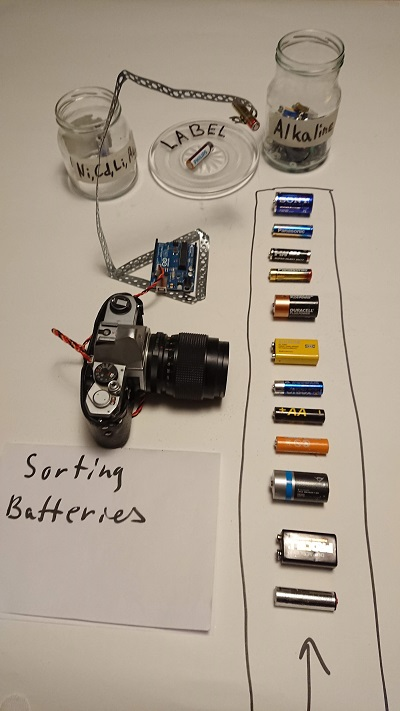
\includegraphics{images/setup.jpg} \emph{A visualisation of the setup,
the batteries moves forward on the conveyer belt, the camera takes
images and decides first if the battery should be labelled and second if
it should be sorted as chargeable (contains Pb,Cd,Ni,Hg) or as an
alkaline battery.}

\hypertarget{exploration-and-explotation}{%
\subsubsection{Exploration and
explotation}\label{exploration-and-explotation}}

We can expect context drift both abrupt when completely new battery
brands enter and also gradually when the design and colouring of brands
change. This indicates that we need a strategy to label some of the
batteries that comes in.

In the \href{https://ieeexplore.ieee.org/document/6414645}{article} we
use as inspiration four strategies are outlined that balance
exploitation and exploration to select batteries to label. We have
implemented two, one random (exploration) and one based on accuracy
(exploitation). Other algorithms combine the strategies and balance
exploration and exploitation.

\hypertarget{metric}{%
\subsubsection{Metric}\label{metric}}

In this example we sort batteries in two classes ``alkaline'' and
``chargeable''. We have used a extremely simplified budget of 10 units
and a labelling cost of 2 units. The budget of course has to be per time
unit and there needs to be penalties for wrongly sorted batteries.

\hypertarget{some-information-around-sorting}{%
\subsubsection{Some information around
sorting}\label{some-information-around-sorting}}

A real world solution that uses machine learning to sort batteries can
be seen here
\href{https://www.youtube.com/watch?feature=player_embedded\&v=OugqnVO7WiU}{film}.
And som infomation around the problem i
\href{https://www.sopor.nu/fakta-om-sopor/vad-haender-med-din-sopa/elavfall/batterier}{general
(in swedish}

    \begin{Verbatim}[commandchars=\\\{\}]
{\color{incolor}In [{\color{incolor}6}]:} \PY{c+c1}{\PYZsh{} Som get started crap run this first}
        \PY{o}{\PYZpc{}}\PY{k}{reload\PYZus{}ext} autoreload
        \PY{o}{\PYZpc{}}\PY{k}{autoreload} 2
        \PY{o}{\PYZpc{}}\PY{k}{matplotlib} inline
        \PY{k+kn}{from} \PY{n+nn}{IPython}\PY{n+nn}{.}\PY{n+nn}{display} \PY{k}{import} \PY{n}{Markdown}\PY{p}{,} \PY{n}{display}
        \PY{k}{def} \PY{n+nf}{printmd}\PY{p}{(}\PY{n}{string}\PY{p}{)}\PY{p}{:}
            \PY{n}{display}\PY{p}{(}\PY{n}{Markdown}\PY{p}{(}\PY{n}{string}\PY{p}{)}\PY{p}{)}
        \PY{k+kn}{import} \PY{n+nn}{sys}
        \PY{k+kn}{import} \PY{n+nn}{zipfile}
        \PY{k+kn}{import} \PY{n+nn}{platform}
        \PY{c+c1}{\PYZsh{}sys.path.append(\PYZdq{}../\PYZdq{})}
        \PY{k+kn}{from} \PY{n+nn}{fastaiold}\PY{n+nn}{.}\PY{n+nn}{imports} \PY{k}{import} \PY{o}{*}
        \PY{n+nb}{print}\PY{p}{(}\PY{n}{platform}\PY{o}{.}\PY{n}{python\PYZus{}version}\PY{p}{(}\PY{p}{)}\PY{p}{)}
        \PY{k+kn}{from} \PY{n+nn}{fastaiold}\PY{n+nn}{.}\PY{n+nn}{transforms} \PY{k}{import} \PY{o}{*}
        \PY{k+kn}{from} \PY{n+nn}{fastaiold}\PY{n+nn}{.}\PY{n+nn}{conv\PYZus{}learner} \PY{k}{import} \PY{o}{*}
        \PY{k+kn}{from} \PY{n+nn}{fastaiold}\PY{n+nn}{.}\PY{n+nn}{model} \PY{k}{import} \PY{o}{*}
        \PY{k+kn}{from} \PY{n+nn}{fastaiold}\PY{n+nn}{.}\PY{n+nn}{dataset} \PY{k}{import} \PY{o}{*}
        \PY{k+kn}{from} \PY{n+nn}{fastaiold}\PY{n+nn}{.}\PY{n+nn}{sgdr} \PY{k}{import} \PY{o}{*}
        \PY{k+kn}{from} \PY{n+nn}{fastaiold}\PY{n+nn}{.}\PY{n+nn}{plots} \PY{k}{import} \PY{o}{*}
        \PY{c+c1}{\PYZsh{} set some variables}
        \PY{c+c1}{\PYZsh{}PATH = \PYZdq{}data/batteries\PYZus{}v1/batteries/\PYZdq{} First version}
        \PY{n}{PATH} \PY{o}{=} \PY{l+s+s2}{\PYZdq{}}\PY{l+s+s2}{data/batteries\PYZus{}v4/}\PY{l+s+s2}{\PYZdq{}}
        \PY{n}{arch}\PY{o}{=}\PY{n}{resnet34}  \PY{c+c1}{\PYZsh{}\PYZsh{}Using the resnet34 model}
        \PY{n}{sz}\PY{o}{=}\PY{l+m+mi}{224}
        \PY{n+nb}{print}\PY{p}{(}\PY{n}{f}\PY{l+s+s1}{\PYZsq{}}\PY{l+s+s1}{NVidia GPUs is called CUDA aviable }\PY{l+s+s1}{\PYZob{}}\PY{l+s+s1}{torch.cuda.is\PYZus{}available()\PYZcb{}}\PY{l+s+s1}{\PYZsq{}}\PY{p}{)}
        \PY{n+nb}{print}\PY{p}{(}\PY{n}{f}\PY{l+s+s1}{\PYZsq{}}\PY{l+s+s1}{deep learning accelerator aviable CuDNN }\PY{l+s+si}{\PYZob{}torch.backends.cudnn.enabled\PYZcb{}}\PY{l+s+s1}{\PYZsq{}}\PY{p}{)}
\end{Verbatim}


    \begin{Verbatim}[commandchars=\\\{\}]
3.6.5
NVidia GPUs is called CUDA aviable True
deep learning accelerator aviable CuDNN True

    \end{Verbatim}

    \hypertarget{utility-functions}{%
\subsection{Utility functions}\label{utility-functions}}

Run this to unpack images that will be used for learning.

    \begin{Verbatim}[commandchars=\\\{\}]
{\color{incolor}In [{\color{incolor}4}]:} \PY{c+c1}{\PYZsh{}Unpack images from zipfile to data lib}
        \PY{c+c1}{\PYZsh{}\PYZpc{} rm \PYZhy{}rf (mydata/tools}
        \PY{k}{with} \PY{n}{zipfile}\PY{o}{.}\PY{n}{ZipFile}\PY{p}{(}\PY{l+s+s2}{\PYZdq{}}\PY{l+s+s2}{data/batteries.zip}\PY{l+s+s2}{\PYZdq{}}\PY{p}{,}\PY{l+s+s2}{\PYZdq{}}\PY{l+s+s2}{r}\PY{l+s+s2}{\PYZdq{}}\PY{p}{)} \PY{k}{as} \PY{n}{zip\PYZus{}ref}\PY{p}{:}
            \PY{n}{zip\PYZus{}ref}\PY{o}{.}\PY{n}{extractall}\PY{p}{(}\PY{l+s+s2}{\PYZdq{}}\PY{l+s+s2}{data/batteries\PYZus{}v1}\PY{l+s+s2}{\PYZdq{}}\PY{p}{)}
\end{Verbatim}


    \hypertarget{train-batteries}{%
\subsection{Train batteries}\label{train-batteries}}

    \begin{Verbatim}[commandchars=\\\{\}]
{\color{incolor}In [{\color{incolor}11}]:} \PY{c+c1}{\PYZsh{} Uncomment below if you need to reset your precomputed activations}
         \PY{c+c1}{\PYZsh{}shutil.rmtree(f\PYZsq{}\PYZob{}PATH\PYZcb{}tmp\PYZsq{}, ignore\PYZus{}errors=True)}
         \PY{n}{data} \PY{o}{=} \PY{n}{ImageClassifierData}\PY{o}{.}\PY{n}{from\PYZus{}paths}\PY{p}{(}\PY{n}{PATH}\PY{p}{,} \PY{n}{tfms}\PY{o}{=}\PY{n}{tfms\PYZus{}from\PYZus{}model}\PY{p}{(}\PY{n}{arch}\PY{p}{,} \PY{n}{sz}\PY{p}{)}\PY{p}{,} \PY{n}{test\PYZus{}name}\PY{o}{=}\PY{l+s+s2}{\PYZdq{}}\PY{l+s+s2}{test}\PY{l+s+s2}{\PYZdq{}}\PY{p}{)}
         \PY{n}{learn} \PY{o}{=} \PY{n}{ConvLearner}\PY{o}{.}\PY{n}{pretrained}\PY{p}{(}\PY{n}{arch}\PY{p}{,} \PY{n}{data}\PY{p}{,} \PY{n}{precompute}\PY{o}{=}\PY{k+kc}{True}\PY{p}{)}
         \PY{n}{learn}\PY{o}{.}\PY{n}{fit}\PY{p}{(}\PY{l+m+mf}{0.01}\PY{p}{,} \PY{l+m+mi}{30}\PY{p}{)}
         \PY{c+c1}{\PYZsh{}prints training loss, validation loss and accuracy}
         \PY{n}{learn}\PY{o}{.}\PY{n}{save}\PY{p}{(}\PY{l+s+s2}{\PYZdq{}}\PY{l+s+s2}{batteries\PYZus{}v4}\PY{l+s+s2}{\PYZdq{}}\PY{p}{)}
\end{Verbatim}


    
    \begin{verbatim}
HBox(children=(IntProgress(value=0, description='Epoch', max=30), HTML(value='')))
    \end{verbatim}

    
    \begin{Verbatim}[commandchars=\\\{\}]
epoch      trn\_loss   val\_loss   accuracy        
    0      0.962626   1.097628   0.241379  
    1      0.825353   0.926875   0.413793        
    2      0.767779   0.692717   0.517241        
    3      0.687022   0.488105   0.758621        
    4      0.590926   0.36693    0.827586        
    5      0.530538   0.29376    0.862069        
    6      0.533866   0.262622   0.862069        
    7      0.525163   0.242112   0.931035        
    8      0.476446   0.248126   0.931035        
    9      0.429491   0.232006   0.931035        
    10     0.387846   0.227366   0.931035        
    11     0.356235   0.224248   0.931035        
    12     0.337142   0.227769   0.931035        
    13     0.309699   0.227071   0.931035        
    14     0.293076   0.215799   0.931035        
    15     0.272245   0.204869   0.931035        
    16     0.255008   0.195808   0.931035        
    17     0.250952   0.18947    0.931035        
    18     0.234087   0.17365    0.931035        
    19     0.218952   0.166069   0.965517        
    20     0.206833   0.162668   0.965517        
    21     0.220964   0.158332   0.965517        
    22     0.209582   0.157056   0.965517        
    23     0.199749   0.139798   0.965517        
    24     0.190355   0.137253   0.965517        
    25     0.182889   0.128084   0.965517        
    26     0.173281   0.123708   0.965517        
    27     0.166457   0.116395   0.965517        
    28     0.158783   0.111196   0.965517        
    29     0.150591   0.105973   0.965517        


    \end{Verbatim}

    \begin{Verbatim}[commandchars=\\\{\}]
{\color{incolor}In [{\color{incolor}49}]:} \PY{c+c1}{\PYZsh{}transforms\PYZus{}top\PYZus{}down, transforms\PYZus{}side\PYZus{}on, transforms\PYZus{}basic }
         \PY{c+c1}{\PYZsh{}shutil.rmtree(f\PYZsq{}\PYZob{}PATH\PYZcb{}tmp\PYZsq{}, ignore\PYZus{}errors=True)}
         \PY{n}{tfms} \PY{o}{=} \PY{n}{tfms\PYZus{}from\PYZus{}model}\PY{p}{(}\PY{n}{resnet34}\PY{p}{,} \PY{n}{sz}\PY{p}{,} \PY{n}{aug\PYZus{}tfms}\PY{o}{=}\PY{n}{transforms\PYZus{}side\PYZus{}on}\PY{p}{,} \PY{n}{max\PYZus{}zoom}\PY{o}{=}\PY{l+m+mf}{1.1}\PY{p}{)}
         \PY{n}{data} \PY{o}{=} \PY{n}{ImageClassifierData}\PY{o}{.}\PY{n}{from\PYZus{}paths}\PY{p}{(}\PY{n}{PATH}\PY{p}{,} \PY{n}{tfms}\PY{o}{=}\PY{n}{tfms}\PY{p}{,} \PY{n}{test\PYZus{}name}\PY{o}{=}\PY{l+s+s1}{\PYZsq{}}\PY{l+s+s1}{test}\PY{l+s+s1}{\PYZsq{}}\PY{p}{)}
         \PY{n}{learn} \PY{o}{=} \PY{n}{ConvLearner}\PY{o}{.}\PY{n}{pretrained}\PY{p}{(}\PY{n}{arch}\PY{p}{,} \PY{n}{data}\PY{p}{,} \PY{n}{precompute}\PY{o}{=}\PY{k+kc}{True}\PY{p}{)}
         \PY{n}{learn}\PY{o}{.}\PY{n}{fit}\PY{p}{(}\PY{l+m+mf}{1e\PYZhy{}2}\PY{p}{,} \PY{l+m+mi}{6}\PY{p}{)}
\end{Verbatim}


    
    \begin{verbatim}
HBox(children=(IntProgress(value=0, description='Epoch', max=6), HTML(value='')))
    \end{verbatim}

    
    \begin{Verbatim}[commandchars=\\\{\}]
epoch      trn\_loss   val\_loss   accuracy        
    0      1.423043   1.209692   0.344828  
    1      1.121907   0.815112   0.448276        
    2      0.861128   0.551593   0.655172        
    3      0.715184   0.409758   0.758621        
    4      0.618384   0.317259   0.896552        
    5      0.569762   0.26605    0.896552        


    \end{Verbatim}

\begin{Verbatim}[commandchars=\\\{\}]
{\color{outcolor}Out[{\color{outcolor}49}]:} [array([0.26605]), 0.8965517282485962]
\end{Verbatim}
            
    \begin{Verbatim}[commandchars=\\\{\}]
{\color{incolor}In [{\color{incolor}8}]:} \PY{n}{learn}\PY{o}{.}\PY{n}{sched}\PY{o}{.}\PY{n}{plot\PYZus{}loss}\PY{p}{(}\PY{p}{)}
\end{Verbatim}


    \begin{center}
    \adjustimage{max size={0.9\linewidth}{0.9\paperheight}}{output_8_0.png}
    \end{center}
    { \hspace*{\fill} \\}
    
    \hypertarget{view-training-and-validation-set-for-batteries}{%
\subsection{View training and validation set for
batteries}\label{view-training-and-validation-set-for-batteries}}

    \begin{Verbatim}[commandchars=\\\{\}]
{\color{incolor}In [{\color{incolor}38}]:} \PY{c+c1}{\PYZsh{} Run to register the plot functions}
         \PY{c+c1}{\PYZsh{}And I know verbose.....}
         \PY{k}{def} \PY{n+nf}{plots}\PY{p}{(}\PY{n}{ims}\PY{p}{,} \PY{n}{figsize}\PY{o}{=}\PY{p}{(}\PY{l+m+mi}{12}\PY{p}{,}\PY{l+m+mi}{6}\PY{p}{)}\PY{p}{,} \PY{n}{rows}\PY{o}{=}\PY{l+m+mi}{1}\PY{p}{,} \PY{n}{titles}\PY{o}{=}\PY{k+kc}{None}\PY{p}{)}\PY{p}{:}
             \PY{n}{f} \PY{o}{=} \PY{n}{plt}\PY{o}{.}\PY{n}{figure}\PY{p}{(}\PY{n}{figsize}\PY{o}{=}\PY{n}{figsize}\PY{p}{)}
             \PY{k}{for} \PY{n}{i} \PY{o+ow}{in} \PY{n+nb}{range}\PY{p}{(}\PY{n+nb}{len}\PY{p}{(}\PY{n}{ims}\PY{p}{)}\PY{p}{)}\PY{p}{:}
                 \PY{k}{try}\PY{p}{:}
                     \PY{n}{sp} \PY{o}{=} \PY{n}{f}\PY{o}{.}\PY{n}{add\PYZus{}subplot}\PY{p}{(}\PY{n}{rows}\PY{p}{,} \PY{n+nb}{len}\PY{p}{(}\PY{n}{ims}\PY{p}{)}\PY{o}{/}\PY{o}{/}\PY{n}{rows}\PY{p}{,} \PY{n}{i}\PY{o}{+}\PY{l+m+mi}{1}\PY{p}{)}
                 \PY{k}{except} \PY{n+ne}{ValueError}\PY{p}{:}
                     \PY{n+nb}{print}\PY{p}{(}\PY{l+s+s2}{\PYZdq{}}\PY{l+s+s2}{\PYZdq{}}\PY{p}{)}
                 \PY{n}{sp}\PY{o}{.}\PY{n}{axis}\PY{p}{(}\PY{l+s+s1}{\PYZsq{}}\PY{l+s+s1}{Off}\PY{l+s+s1}{\PYZsq{}}\PY{p}{)}
                 \PY{k}{if} \PY{n}{titles} \PY{o+ow}{is} \PY{o+ow}{not} \PY{k+kc}{None}\PY{p}{:} \PY{n}{sp}\PY{o}{.}\PY{n}{set\PYZus{}title}\PY{p}{(}\PY{n}{titles}\PY{p}{[}\PY{n}{i}\PY{p}{]}\PY{p}{,} \PY{n}{fontsize}\PY{o}{=}\PY{l+m+mi}{16}\PY{p}{)}
                 \PY{n}{plt}\PY{o}{.}\PY{n}{imshow}\PY{p}{(}\PY{n}{ims}\PY{p}{[}\PY{n}{i}\PY{p}{]}\PY{p}{)}
                 
         \PY{k}{def} \PY{n+nf}{plot\PYZus{}images\PYZus{}from\PYZus{}train\PYZus{}set}\PY{p}{(}\PY{n}{train\PYZus{}y}\PY{p}{)}\PY{p}{:}
             \PY{n}{imgs}\PY{o}{=}\PY{p}{[}\PY{p}{]}
             \PY{n}{titles}\PY{o}{=}\PY{p}{[}\PY{p}{]}
             \PY{n}{res} \PY{o}{=} \PY{n}{np}\PY{o}{.}\PY{n}{extract}\PY{p}{(}\PY{n}{data}\PY{o}{.}\PY{n}{trn\PYZus{}y}\PY{o}{==}\PY{n}{train\PYZus{}y}\PY{p}{,}\PY{n}{data}\PY{o}{.}\PY{n}{trn\PYZus{}ds}\PY{o}{.}\PY{n}{fnames}\PY{p}{)}
             \PY{n}{printmd}\PY{p}{(}\PY{l+s+s2}{\PYZdq{}}\PY{l+s+s2}{\PYZsh{} }\PY{l+s+s2}{\PYZdq{}}\PY{o}{+}\PY{n}{data}\PY{o}{.}\PY{n}{classes}\PY{p}{[}\PY{n}{train\PYZus{}y}\PY{p}{]}\PY{o}{+}\PY{l+s+s2}{\PYZdq{}}\PY{l+s+s2}{s in training set}\PY{l+s+s2}{\PYZdq{}}\PY{p}{)}
             \PY{k}{for} \PY{n}{i} \PY{o+ow}{in} \PY{n+nb}{range}\PY{p}{(}\PY{l+m+mi}{0}\PY{p}{,}\PY{n+nb}{len}\PY{p}{(}\PY{n}{res}\PY{p}{)}\PY{p}{)}\PY{p}{:}
                 \PY{n}{title} \PY{o}{=} \PY{n}{res}\PY{p}{[}\PY{n}{i}\PY{p}{]}
                 \PY{c+c1}{\PYZsh{}print(title)}
                 \PY{n}{imgs}\PY{o}{.}\PY{n}{append}\PY{p}{(}\PY{n}{plt}\PY{o}{.}\PY{n}{imread}\PY{p}{(}\PY{n}{PATH} \PY{o}{+} \PY{n}{res}\PY{p}{[}\PY{n}{i}\PY{p}{]}\PY{p}{)}\PY{p}{)}
                 \PY{n}{titles}\PY{o}{.}\PY{n}{append}\PY{p}{(}\PY{n}{title}\PY{p}{)}    
             \PY{k}{return} \PY{n}{plots}\PY{p}{(}\PY{n}{imgs}\PY{p}{,}\PY{n}{titles}\PY{o}{=}\PY{n}{titles}\PY{p}{,}\PY{n}{rows}\PY{o}{=}\PY{l+m+mi}{10}\PY{p}{,}\PY{n}{figsize}\PY{o}{=}\PY{p}{(}\PY{l+m+mi}{20}\PY{p}{,}\PY{l+m+mi}{16}\PY{p}{)}\PY{p}{)}
         
         \PY{k}{def} \PY{n+nf}{plot\PYZus{}images\PYZus{}from\PYZus{}val\PYZus{}set}\PY{p}{(}\PY{n}{val\PYZus{}y}\PY{p}{)}\PY{p}{:}
             \PY{n}{imgs}\PY{o}{=}\PY{p}{[}\PY{p}{]}
             \PY{n}{titles}\PY{o}{=}\PY{p}{[}\PY{p}{]}
             \PY{n}{res} \PY{o}{=} \PY{n}{np}\PY{o}{.}\PY{n}{extract}\PY{p}{(}\PY{n}{data}\PY{o}{.}\PY{n}{val\PYZus{}y}\PY{o}{==}\PY{n}{val\PYZus{}y}\PY{p}{,}\PY{n}{data}\PY{o}{.}\PY{n}{val\PYZus{}ds}\PY{o}{.}\PY{n}{fnames}\PY{p}{)}
             \PY{n}{printmd}\PY{p}{(}\PY{l+s+s2}{\PYZdq{}}\PY{l+s+s2}{\PYZsh{} }\PY{l+s+s2}{\PYZdq{}}\PY{o}{+}\PY{n}{data}\PY{o}{.}\PY{n}{classes}\PY{p}{[}\PY{n}{val\PYZus{}y}\PY{p}{]}\PY{o}{+}\PY{l+s+s2}{\PYZdq{}}\PY{l+s+s2}{s in validation set}\PY{l+s+s2}{\PYZdq{}}\PY{p}{)}
             \PY{k}{for} \PY{n}{i} \PY{o+ow}{in} \PY{n+nb}{range}\PY{p}{(}\PY{l+m+mi}{0}\PY{p}{,}\PY{n+nb}{len}\PY{p}{(}\PY{n}{res}\PY{p}{)}\PY{p}{)}\PY{p}{:}
                 \PY{n}{title} \PY{o}{=} \PY{n}{res}\PY{p}{[}\PY{n}{i}\PY{p}{]}
                 \PY{c+c1}{\PYZsh{}print(title)}
                 \PY{n}{imgs}\PY{o}{.}\PY{n}{append}\PY{p}{(}\PY{n}{plt}\PY{o}{.}\PY{n}{imread}\PY{p}{(}\PY{n}{PATH} \PY{o}{+} \PY{n}{res}\PY{p}{[}\PY{n}{i}\PY{p}{]}\PY{p}{)}\PY{p}{)}
                 \PY{n}{titles}\PY{o}{.}\PY{n}{append}\PY{p}{(}\PY{n}{title}\PY{p}{)}    
             \PY{k}{return} \PY{n}{plots}\PY{p}{(}\PY{n}{imgs}\PY{p}{,}\PY{n}{titles}\PY{o}{=}\PY{n}{titles}\PY{p}{,}\PY{n}{rows}\PY{o}{=}\PY{l+m+mi}{5}\PY{p}{,}\PY{n}{figsize}\PY{o}{=}\PY{p}{(}\PY{l+m+mi}{16}\PY{p}{,}\PY{l+m+mi}{8}\PY{p}{)}\PY{p}{)}
         
         \PY{c+c1}{\PYZsh{}print(\PYZdq{}The classes: \PYZdq{}+str(data.classes))}
         \PY{c+c1}{\PYZsh{}print(\PYZdq{}And the validation set alkaline is 0 and chargeable is 1:\PYZdq{} +str(data.val\PYZus{}y))}
\end{Verbatim}


    \begin{Verbatim}[commandchars=\\\{\}]
{\color{incolor}In [{\color{incolor}29}]:} \PY{c+c1}{\PYZsh{}Alkalines}
         \PY{n}{plot\PYZus{}images\PYZus{}from\PYZus{}train\PYZus{}set}\PY{p}{(}\PY{l+m+mi}{0}\PY{p}{)}
\end{Verbatim}


    \hypertarget{alkalines-in-training-set}{%
\section{alkalines in training set}\label{alkalines-in-training-set}}

    
    \begin{Verbatim}[commandchars=\\\{\}]








    \end{Verbatim}

    \begin{center}
    \adjustimage{max size={0.9\linewidth}{0.9\paperheight}}{output_11_2.png}
    \end{center}
    { \hspace*{\fill} \\}
    
    \begin{Verbatim}[commandchars=\\\{\}]
{\color{incolor}In [{\color{incolor}25}]:} \PY{c+c1}{\PYZsh{}Chargeables}
         \PY{n}{plot\PYZus{}images\PYZus{}from\PYZus{}train\PYZus{}set}\PY{p}{(}\PY{l+m+mi}{1}\PY{p}{)}
\end{Verbatim}


    \hypertarget{chargeables-in-training-set}{%
\section{chargeables in training
set}\label{chargeables-in-training-set}}

    
    \begin{Verbatim}[commandchars=\\\{\}]


    \end{Verbatim}

    \begin{center}
    \adjustimage{max size={0.9\linewidth}{0.9\paperheight}}{output_12_2.png}
    \end{center}
    { \hspace*{\fill} \\}
    
    \begin{Verbatim}[commandchars=\\\{\}]
{\color{incolor}In [{\color{incolor}26}]:} \PY{c+c1}{\PYZsh{}Alkalines}
         \PY{n}{plot\PYZus{}images\PYZus{}from\PYZus{}val\PYZus{}set}\PY{p}{(}\PY{l+m+mi}{0}\PY{p}{)}
\end{Verbatim}


    \hypertarget{alkalines-in-validation-set}{%
\section{alkalines in validation
set}\label{alkalines-in-validation-set}}

    
    \begin{Verbatim}[commandchars=\\\{\}]



    \end{Verbatim}

    \begin{center}
    \adjustimage{max size={0.9\linewidth}{0.9\paperheight}}{output_13_2.png}
    \end{center}
    { \hspace*{\fill} \\}
    
    \begin{Verbatim}[commandchars=\\\{\}]
{\color{incolor}In [{\color{incolor}30}]:} \PY{c+c1}{\PYZsh{}Chargeables}
         \PY{n}{plot\PYZus{}images\PYZus{}from\PYZus{}val\PYZus{}set}\PY{p}{(}\PY{l+m+mi}{1}\PY{p}{)}
\end{Verbatim}


    \hypertarget{chargeables-in-validation-set}{%
\section{chargeables in validation
set}\label{chargeables-in-validation-set}}

    
    \begin{Verbatim}[commandchars=\\\{\}]



    \end{Verbatim}

    \begin{center}
    \adjustimage{max size={0.9\linewidth}{0.9\paperheight}}{output_14_2.png}
    \end{center}
    { \hspace*{\fill} \\}
    
    \hypertarget{confusion-matrix}{%
\subsection{Confusion matrix}\label{confusion-matrix}}

    \begin{Verbatim}[commandchars=\\\{\}]
{\color{incolor}In [{\color{incolor}9}]:} \PY{n}{log\PYZus{}preds}\PY{p}{,}\PY{n}{y} \PY{o}{=} \PY{n}{learn}\PY{o}{.}\PY{n}{TTA}\PY{p}{(}\PY{p}{)}
        \PY{n}{probs} \PY{o}{=} \PY{n}{np}\PY{o}{.}\PY{n}{mean}\PY{p}{(}\PY{n}{np}\PY{o}{.}\PY{n}{exp}\PY{p}{(}\PY{n}{log\PYZus{}preds}\PY{p}{)}\PY{p}{,}\PY{l+m+mi}{0}\PY{p}{)}
        \PY{n+nb}{print}\PY{p}{(}\PY{l+s+s2}{\PYZdq{}}\PY{l+s+s2}{Accurracy validation set: }\PY{l+s+s2}{\PYZdq{}}\PY{o}{+}\PY{n+nb}{str}\PY{p}{(}\PY{n}{np}\PY{o}{.}\PY{n}{around}\PY{p}{(}\PY{n}{accuracy\PYZus{}np}\PY{p}{(}\PY{n}{probs}\PY{p}{,} \PY{n}{y}\PY{p}{)}\PY{p}{,}\PY{n}{decimals}\PY{o}{=}\PY{l+m+mi}{2}\PY{p}{)}\PY{p}{)}\PY{p}{)}
        \PY{n}{preds} \PY{o}{=} \PY{n}{np}\PY{o}{.}\PY{n}{argmax}\PY{p}{(}\PY{n}{probs}\PY{p}{,} \PY{n}{axis}\PY{o}{=}\PY{l+m+mi}{1}\PY{p}{)}
        \PY{n}{probs} \PY{o}{=} \PY{n}{probs}\PY{p}{[}\PY{p}{:}\PY{p}{,}\PY{l+m+mi}{1}\PY{p}{]}
        \PY{k+kn}{from} \PY{n+nn}{sklearn}\PY{n+nn}{.}\PY{n+nn}{metrics} \PY{k}{import} \PY{n}{confusion\PYZus{}matrix}
        \PY{c+c1}{\PYZsh{}accuracy\PYZus{}np(probs, y)}
        \PY{n}{cm} \PY{o}{=} \PY{n}{confusion\PYZus{}matrix}\PY{p}{(}\PY{n}{y}\PY{p}{,} \PY{n}{preds}\PY{p}{)}
        \PY{c+c1}{\PYZsh{}Recall = how many correct among the ones in the bin (ideally max 1)}
        \PY{n+nb}{print}\PY{p}{(}\PY{l+s+s2}{\PYZdq{}}\PY{l+s+s2}{Recall for alkaline: }\PY{l+s+s2}{\PYZdq{}}\PY{o}{+}\PY{n+nb}{str}\PY{p}{(}\PY{n}{np}\PY{o}{.}\PY{n}{around}\PY{p}{(}\PY{n}{cm}\PY{p}{[}\PY{l+m+mi}{0}\PY{p}{,}\PY{l+m+mi}{0}\PY{p}{]}\PY{o}{/}\PY{p}{(}\PY{n}{cm}\PY{p}{[}\PY{l+m+mi}{0}\PY{p}{,}\PY{l+m+mi}{1}\PY{p}{]}\PY{o}{+}\PY{n}{cm}\PY{p}{[}\PY{l+m+mi}{0}\PY{p}{,}\PY{l+m+mi}{0}\PY{p}{]}\PY{p}{)}\PY{p}{,}\PY{n}{decimals}\PY{o}{=}\PY{l+m+mi}{2}\PY{p}{)}\PY{p}{)}\PY{p}{)}
        \PY{c+c1}{\PYZsh{}Recall = how many correct classified among all that should be among all correct (ideally max 1).}
        \PY{n+nb}{print}\PY{p}{(}\PY{l+s+s2}{\PYZdq{}}\PY{l+s+s2}{Precision for alkaline: }\PY{l+s+s2}{\PYZdq{}}\PY{o}{+}\PY{n+nb}{str}\PY{p}{(}\PY{n}{np}\PY{o}{.}\PY{n}{around}\PY{p}{(}\PY{n}{cm}\PY{p}{[}\PY{l+m+mi}{0}\PY{p}{,}\PY{l+m+mi}{0}\PY{p}{]}\PY{o}{/}\PY{p}{(}\PY{n}{cm}\PY{p}{[}\PY{l+m+mi}{0}\PY{p}{,}\PY{l+m+mi}{0}\PY{p}{]}\PY{o}{+}\PY{n}{cm}\PY{p}{[}\PY{l+m+mi}{1}\PY{p}{,}\PY{l+m+mi}{0}\PY{p}{]}\PY{p}{)}\PY{p}{,}\PY{n}{decimals}\PY{o}{=}\PY{l+m+mi}{2}\PY{p}{)}\PY{p}{)}\PY{p}{)}
        \PY{n+nb}{print}\PY{p}{(}\PY{l+s+s2}{\PYZdq{}}\PY{l+s+s2}{Recall for chargeable: }\PY{l+s+s2}{\PYZdq{}}\PY{o}{+}\PY{n+nb}{str}\PY{p}{(}\PY{n}{np}\PY{o}{.}\PY{n}{around}\PY{p}{(}\PY{n}{cm}\PY{p}{[}\PY{l+m+mi}{1}\PY{p}{,}\PY{l+m+mi}{1}\PY{p}{]}\PY{o}{/}\PY{p}{(}\PY{n}{cm}\PY{p}{[}\PY{l+m+mi}{1}\PY{p}{,}\PY{l+m+mi}{1}\PY{p}{]}\PY{o}{+}\PY{n}{cm}\PY{p}{[}\PY{l+m+mi}{1}\PY{p}{,}\PY{l+m+mi}{0}\PY{p}{]}\PY{p}{)}\PY{p}{,}\PY{n}{decimals}\PY{o}{=}\PY{l+m+mi}{2}\PY{p}{)}\PY{p}{)}\PY{p}{)}
        \PY{n+nb}{print}\PY{p}{(}\PY{l+s+s2}{\PYZdq{}}\PY{l+s+s2}{Precision for chargeable: }\PY{l+s+s2}{\PYZdq{}}\PY{o}{+}\PY{n+nb}{str}\PY{p}{(}\PY{n}{np}\PY{o}{.}\PY{n}{around}\PY{p}{(}\PY{n}{cm}\PY{p}{[}\PY{l+m+mi}{1}\PY{p}{,}\PY{l+m+mi}{1}\PY{p}{]}\PY{o}{/}\PY{p}{(}\PY{n}{cm}\PY{p}{[}\PY{l+m+mi}{1}\PY{p}{,}\PY{l+m+mi}{1}\PY{p}{]}\PY{o}{+}\PY{n}{cm}\PY{p}{[}\PY{l+m+mi}{0}\PY{p}{,}\PY{l+m+mi}{1}\PY{p}{]}\PY{p}{)}\PY{p}{,}\PY{n}{decimals}\PY{o}{=}\PY{l+m+mi}{2}\PY{p}{)}\PY{p}{)}\PY{p}{)}
        \PY{n}{plot\PYZus{}confusion\PYZus{}matrix}\PY{p}{(}\PY{n}{cm}\PY{p}{,} \PY{n}{data}\PY{o}{.}\PY{n}{classes}\PY{p}{)}
        
        \PY{n}{wrong\PYZus{}validation}\PY{o}{=}\PY{n}{np}\PY{o}{.}\PY{n}{where}\PY{p}{(}\PY{n}{np}\PY{o}{.}\PY{n}{add}\PY{p}{(}\PY{n}{y}\PY{p}{,}\PY{n}{preds}\PY{p}{)} \PY{o}{==} \PY{l+m+mi}{1}\PY{p}{)}\PY{p}{[}\PY{l+m+mi}{0}\PY{p}{]}
        
        \PY{k}{def} \PY{n+nf}{plots}\PY{p}{(}\PY{n}{ims}\PY{p}{,} \PY{n}{figsize}\PY{o}{=}\PY{p}{(}\PY{l+m+mi}{12}\PY{p}{,}\PY{l+m+mi}{6}\PY{p}{)}\PY{p}{,} \PY{n}{rows}\PY{o}{=}\PY{l+m+mi}{1}\PY{p}{,} \PY{n}{titles}\PY{o}{=}\PY{k+kc}{None}\PY{p}{)}\PY{p}{:}
            \PY{n}{f} \PY{o}{=} \PY{n}{plt}\PY{o}{.}\PY{n}{figure}\PY{p}{(}\PY{n}{figsize}\PY{o}{=}\PY{n}{figsize}\PY{p}{)}
            \PY{k}{for} \PY{n}{i} \PY{o+ow}{in} \PY{n+nb}{range}\PY{p}{(}\PY{n+nb}{len}\PY{p}{(}\PY{n}{ims}\PY{p}{)}\PY{p}{)}\PY{p}{:}
                \PY{k}{try}\PY{p}{:}
                    \PY{n}{sp} \PY{o}{=} \PY{n}{f}\PY{o}{.}\PY{n}{add\PYZus{}subplot}\PY{p}{(}\PY{n}{rows}\PY{p}{,} \PY{n+nb}{len}\PY{p}{(}\PY{n}{ims}\PY{p}{)}\PY{o}{/}\PY{o}{/}\PY{n}{rows}\PY{p}{,} \PY{n}{i}\PY{o}{+}\PY{l+m+mi}{1}\PY{p}{)}
                \PY{k}{except} \PY{n+ne}{ValueError}\PY{p}{:}
                    \PY{n+nb}{print}\PY{p}{(}\PY{l+s+s2}{\PYZdq{}}\PY{l+s+s2}{\PYZdq{}}\PY{p}{)}
                \PY{n}{sp}\PY{o}{.}\PY{n}{axis}\PY{p}{(}\PY{l+s+s1}{\PYZsq{}}\PY{l+s+s1}{Off}\PY{l+s+s1}{\PYZsq{}}\PY{p}{)}
                \PY{k}{if} \PY{n}{titles} \PY{o+ow}{is} \PY{o+ow}{not} \PY{k+kc}{None}\PY{p}{:} \PY{n}{sp}\PY{o}{.}\PY{n}{set\PYZus{}title}\PY{p}{(}\PY{n}{titles}\PY{p}{[}\PY{n}{i}\PY{p}{]}\PY{p}{,} \PY{n}{fontsize}\PY{o}{=}\PY{l+m+mi}{16}\PY{p}{)}
                \PY{n}{plt}\PY{o}{.}\PY{n}{imshow}\PY{p}{(}\PY{n}{ims}\PY{p}{[}\PY{n}{i}\PY{p}{]}\PY{p}{)}
        
        \PY{k}{def} \PY{n+nf}{print\PYZus{}wrong\PYZus{}validation}\PY{p}{(}\PY{p}{)}\PY{p}{:}
            \PY{n}{img} \PY{o}{=} \PY{p}{[}\PY{p}{]}
            \PY{n}{titles} \PY{o}{=} \PY{p}{[}\PY{p}{]}
            \PY{k}{for} \PY{n}{i} \PY{o+ow}{in} \PY{n+nb}{range} \PY{p}{(}\PY{l+m+mi}{0}\PY{p}{,}\PY{n+nb}{len}\PY{p}{(}\PY{n}{wrong\PYZus{}validation}\PY{p}{)}\PY{p}{)}\PY{p}{:}
                \PY{n}{path} \PY{o}{=} \PY{n}{PATH} \PY{o}{+}\PY{n}{data}\PY{o}{.}\PY{n}{val\PYZus{}ds}\PY{o}{.}\PY{n}{fnames}\PY{p}{[}\PY{n}{wrong\PYZus{}validation}\PY{p}{[}\PY{n}{i}\PY{p}{]}\PY{p}{]}
                \PY{n}{img}\PY{o}{.}\PY{n}{append}\PY{p}{(}\PY{n}{plt}\PY{o}{.}\PY{n}{imread}\PY{p}{(}\PY{n}{path}\PY{p}{)}\PY{p}{)}
                \PY{n}{titles}\PY{o}{.}\PY{n}{append}\PY{p}{(}\PY{n}{data}\PY{o}{.}\PY{n}{val\PYZus{}ds}\PY{o}{.}\PY{n}{fnames}\PY{p}{[}\PY{n}{wrong\PYZus{}validation}\PY{p}{[}\PY{n}{i}\PY{p}{]}\PY{p}{]}\PY{o}{+}\PY{l+s+s2}{\PYZdq{}}\PY{l+s+s2}{:}\PY{l+s+s2}{\PYZdq{}}\PY{o}{+}\PY{n}{data}\PY{o}{.}\PY{n}{classes}\PY{p}{[}\PY{n}{preds}\PY{p}{[}\PY{n}{wrong\PYZus{}validation}\PY{p}{[}\PY{n}{i}\PY{p}{]}\PY{p}{]}\PY{p}{]}\PY{p}{)}
                \PY{c+c1}{\PYZsh{}print (data.val\PYZus{}ds.fnames[wrong\PYZus{}validation[i]]+\PYZdq{}:\PYZdq{}+data.classes[y[wrong\PYZus{}validation[i]]])}
                \PY{c+c1}{\PYZsh{}print(\PYZdq{}Classified as: \PYZdq{}+data.classes[preds[wrong\PYZus{}validation[i]]]+\PYZdq{} should be \PYZdq{}+data.classes[y[wrong\PYZus{}validation[i]]])}
            \PY{n}{plots}\PY{p}{(}\PY{n}{img}\PY{p}{,}\PY{n}{titles}\PY{o}{=}\PY{n}{titles}\PY{p}{,}\PY{n}{rows}\PY{o}{=}\PY{l+m+mi}{1}\PY{p}{,}\PY{n}{figsize}\PY{o}{=}\PY{p}{(}\PY{l+m+mi}{20}\PY{p}{,}\PY{l+m+mi}{14}\PY{p}{)}\PY{p}{)}
        
        \PY{n}{print\PYZus{}wrong\PYZus{}validation}\PY{p}{(}\PY{p}{)}    
\end{Verbatim}


    \begin{Verbatim}[commandchars=\\\{\}]
Accurracy validation set: 0.93       
Recall for alkaline: 0.95
Precision for alkaline: 0.95
Recall for chargeable: 0.86
Precision for chargeable: 0.86
[[21  1]
 [ 1  6]]

    \end{Verbatim}

    \begin{center}
    \adjustimage{max size={0.9\linewidth}{0.9\paperheight}}{output_16_1.png}
    \end{center}
    { \hspace*{\fill} \\}
    
    \begin{center}
    \adjustimage{max size={0.9\linewidth}{0.9\paperheight}}{output_16_2.png}
    \end{center}
    { \hspace*{\fill} \\}
    
    \hypertarget{predictions-on-test-set}{%
\subsection{Predictions on test set}\label{predictions-on-test-set}}

Sorted in accuracy order, closer to 0 the model belives it is a
alkaline, closer to 1 the model belives it is a chargeable battery. So
now we will know if it overfitted or included variance/bias.

    \begin{Verbatim}[commandchars=\\\{\}]
{\color{incolor}In [{\color{incolor}10}]:} \PY{k}{def} \PY{n+nf}{plot\PYZus{}predictions\PYZus{}in\PYZus{}accuacy\PYZus{}order}\PY{p}{(}\PY{p}{)}\PY{p}{:}
             \PY{n}{log\PYZus{}preds}\PY{o}{=}\PY{n}{learn}\PY{o}{.}\PY{n}{predict}\PY{p}{(}\PY{n}{is\PYZus{}test}\PY{o}{=}\PY{k+kc}{True}\PY{p}{)} 
             \PY{c+c1}{\PYZsh{}probs = np.round(np.exp(log\PYZus{}preds[:,1])*100,decimals=0) \PYZsh{}\PYZsh{}Convert result from log scale (probs given in log...)}
             \PY{n}{probs} \PY{o}{=} \PY{n}{np}\PY{o}{.}\PY{n}{exp}\PY{p}{(}\PY{n}{log\PYZus{}preds}\PY{p}{[}\PY{p}{:}\PY{p}{,}\PY{l+m+mi}{1}\PY{p}{]}\PY{p}{)}
             \PY{n}{names} \PY{o}{=} \PY{n}{data}\PY{o}{.}\PY{n}{test\PYZus{}ds}\PY{o}{.}\PY{n}{fnames}
             \PY{n}{probs\PYZus{}sorted} \PY{o}{=} \PY{n}{np}\PY{o}{.}\PY{n}{sort}\PY{p}{(}\PY{n}{probs}\PY{p}{)}
             \PY{c+c1}{\PYZsh{}print(probs)}
             \PY{c+c1}{\PYZsh{}print(names)}
             \PY{n}{img\PYZus{}names\PYZus{}sorted\PYZus{}on\PYZus{}probs} \PY{o}{=} \PY{p}{[}\PY{n}{x} \PY{k}{for} \PY{n}{\PYZus{}}\PY{p}{,}\PY{n}{x} \PY{o+ow}{in} \PY{n+nb}{sorted}\PY{p}{(}\PY{n+nb}{zip}\PY{p}{(}\PY{n}{probs}\PY{p}{,}\PY{n}{names}\PY{p}{)}\PY{p}{)}\PY{p}{]}
             \PY{n}{img} \PY{o}{=} \PY{p}{[}\PY{p}{]}
             \PY{n}{titles} \PY{o}{=} \PY{p}{[}\PY{p}{]}
             \PY{k}{for} \PY{n}{i} \PY{o+ow}{in} \PY{n+nb}{range}\PY{p}{(}\PY{l+m+mi}{0}\PY{p}{,}\PY{n+nb}{len}\PY{p}{(}\PY{n}{data}\PY{o}{.}\PY{n}{test\PYZus{}ds}\PY{o}{.}\PY{n}{fnames}\PY{p}{)}\PY{p}{)}\PY{p}{:}
             \PY{c+c1}{\PYZsh{}for i in range(0,4):}
                 \PY{n}{title} \PY{o}{=} \PY{n}{PATH} \PY{o}{+} \PY{n}{img\PYZus{}names\PYZus{}sorted\PYZus{}on\PYZus{}probs}\PY{p}{[}\PY{n}{i}\PY{p}{]}
                 \PY{n}{img}\PY{o}{.}\PY{n}{append}\PY{p}{(}\PY{n}{plt}\PY{o}{.}\PY{n}{imread}\PY{p}{(}\PY{n}{title}\PY{p}{)}\PY{p}{)}
                 \PY{n}{titles}\PY{o}{.}\PY{n}{append}\PY{p}{(}\PY{n}{data}\PY{o}{.}\PY{n}{classes}\PY{p}{[}\PY{n+nb}{int}\PY{p}{(}\PY{n}{probs\PYZus{}sorted}\PY{p}{[}\PY{n}{i}\PY{p}{]}\PY{o}{+}\PY{l+m+mf}{0.5}\PY{p}{)}\PY{p}{]}\PY{o}{+}\PY{l+s+s2}{\PYZdq{}}\PY{l+s+s2}{:}\PY{l+s+s2}{\PYZdq{}}\PY{o}{+}\PY{n+nb}{str}\PY{p}{(}\PY{n}{np}\PY{o}{.}\PY{n}{around}\PY{p}{(}\PY{n}{probs\PYZus{}sorted}\PY{p}{[}\PY{n}{i}\PY{p}{]}\PY{p}{,}\PY{n}{decimals}\PY{o}{=}\PY{l+m+mi}{2}\PY{p}{)}\PY{p}{)}\PY{o}{+}\PY{l+s+s2}{\PYZdq{}}\PY{l+s+s2}{:}\PY{l+s+s2}{\PYZdq{}}\PY{o}{+}\PY{n}{img\PYZus{}names\PYZus{}sorted\PYZus{}on\PYZus{}probs}\PY{p}{[}\PY{n}{i}\PY{p}{]}\PY{p}{)}    
             \PY{k}{return} \PY{n}{plots}\PY{p}{(}\PY{n}{img}\PY{p}{,}\PY{n}{titles}\PY{o}{=}\PY{n}{titles}\PY{p}{,}\PY{n}{rows}\PY{o}{=}\PY{l+m+mi}{5}\PY{p}{,}\PY{n}{figsize}\PY{o}{=}\PY{p}{(}\PY{l+m+mi}{20}\PY{p}{,}\PY{l+m+mi}{16}\PY{p}{)}\PY{p}{)}
         
         \PY{n}{plot\PYZus{}predictions\PYZus{}in\PYZus{}accuacy\PYZus{}order}\PY{p}{(}\PY{p}{)}
\end{Verbatim}


    \begin{Verbatim}[commandchars=\\\{\}]


    \end{Verbatim}

    \begin{center}
    \adjustimage{max size={0.9\linewidth}{0.9\paperheight}}{output_18_1.png}
    \end{center}
    { \hspace*{\fill} \\}
    
    \begin{Verbatim}[commandchars=\\\{\}]
{\color{incolor}In [{\color{incolor} }]:} \PY{c+c1}{\PYZsh{}Unpack images from zipfile to data lib}
        \PY{c+c1}{\PYZsh{}\PYZpc{} rm \PYZhy{}rf (mydata/tools}
        \PY{k}{with} \PY{n}{zipfile}\PY{o}{.}\PY{n}{ZipFile}\PY{p}{(}\PY{l+s+s2}{\PYZdq{}}\PY{l+s+s2}{data/batteries\PYZus{}v4.zip}\PY{l+s+s2}{\PYZdq{}}\PY{p}{,}\PY{l+s+s2}{\PYZdq{}}\PY{l+s+s2}{r}\PY{l+s+s2}{\PYZdq{}}\PY{p}{)} \PY{k}{as} \PY{n}{zip\PYZus{}ref}\PY{p}{:}
            \PY{n}{zip\PYZus{}ref}\PY{o}{.}\PY{n}{extractall}\PY{p}{(}\PY{l+s+s2}{\PYZdq{}}\PY{l+s+s2}{data/}\PY{l+s+s2}{\PYZdq{}}\PY{p}{)}
\end{Verbatim}



    % Add a bibliography block to the postdoc
    
    
    
    \end{document}
